\chapter{Introduction}
\label{chp_1_introduction}

Deep Neural Networks (DNNs), as one of the most prominent models in Artificial Intelligence (AI), have captured global attention. DNNs have transformed numerous fields, including medical biology \cite{zitnik2019machine}, renewable energy \cite{gensler2016deep}, and autonomous vehicles \cite{tian2018deeptest}, by enabling complex and intelligent tasks that were once impractical or unattainable. Achieving high performance in DNNs relies heavily on massive matrix multiplications, demanding substantial computational power. General-purpose processors are not optimized for such tasks, leading to high energy consumption, prolonged execution times, and limited scalability. In response, hardware manufacturers have developed domain-specific hardware, known as AI processors \cite{Dojo, DBLP:conf/isca/JouppiK0MNNPSST23, Mi300, H100, DBLP:conf/isscc/OuyangDML21, DBLP:conf/hotchips/LiaoTXZ19, 910}, which include specialized units to accelerate AI computations. Most of these units are designed to optimize matrix multiplications, known as matrix multiplier-accumulators (MACs), which substantially enhance DNN performance by reducing the execution time for these operations.

Beyond matrix multiplications, complete AI applications also involve various other algorithms and operations, such as the Top-K algorithm used in K-Nearest Neighbors (KNN) \cite{1053964} and Taylor expansions in DNNs \cite{DBLP:conf/cvpr/JinYWMH23}. Compared to matrix multiplications, AI processors typically offer less robust support for scalar or vector operations in terms of (1) quantity (e.g., only one 256-bit vector unit per core in Huawei Ascend processors \cite{DBLP:conf/hotchips/LiaoTXZ19}); (2) computational power (e.g., 22 TFLOPS for FP32 vector units versus 362 TFLOPS for BF16/CFP8 Matrix MACs in Tesla Dojo \cite{Dojo}); and (3) microarchitecture (e.g., the absence of sophisticated features like branch prediction, speculative prefetching, caches, and address coalescing in TPUs \cite{DBLP:conf/isca/JouppiYPPABBBBB17}). These design choices and trade-offs in AI processors have a substantial impact on algorithm optimization. Therefore, an in-depth understanding of the hardware structure and performance characteristics is essential. This thesis examines Huawei Ascend processors \cite{DBLP:conf/hotchips/LiaoTXZ19} as a case study, thoroughly analyzing its architecture and proposing targeted hardware-aware algorithm optimization techniques.

Huawei Ascend architecture \cite{DBLP:conf/hotchips/LiaoTXZ19} introduces a novel approach to AI processing. Huawei has released two versions of the Ascend processor: the Ascend 310 for edge devices \cite{DBLP:conf/hotchips/LiaoTXZ19} and the Ascend 910B for data center servers \cite{910}. Both feature the DaVinci Core, which provides up to 4 TFLOPS of FP16 computational power for matrix multiplications per core. Recently, Huawei also introduced a comprehensive framework called CANN \cite{CANN}, allowing developers to design custom DNN operators on Ascend processors, thereby enabling algorithm-specific optimizations \cite{DBLP:conf/ipps/RohwedderCAACW21, DBLP:conf/icpp/JiW21}. However, without a precise performance model that captures the working details and implications, optimizing algorithms for this novel hardware remains challenging.

To address this, the thesis first presents Verrocchio, a performance model specifically designed for the DaVinci Core of Huawei Ascend AI processors. Verrocchio predicts execution times for Ascend Cube-based Compute Engine (CCE) instructions using discrete-event simulation based on a given kernel program. In developing this model, we perform not only standard benchmarks for individual hardware unit performance but also micro-benchmarks to explore bandwidth contention along data paths. The results of this performance model and benchmarking reveal a critical design trade-off in AI processors: substantial performance gains in Matrix MACs come at the expense of reduced support for other essential operations, such as IO, vector, and scalar operations. As a result, applications that require diverse operations, beyond matrix multiplications, often suffer performance limitations, especially in adapting non-DNN applications.

Taking into account these specific hardware characteristics, this thesis proposes two key approaches for hardware-aware algorithm optimization on AI processors. The first approach involves replacing inefficient scalar and vector operations with alternative scalar and vector operations. Benchmark results indicate that scalar operations exhibit similar low performance across the board, while vectorized comparisons and selections are the most costly. To demonstrate this approach, we introduce SelB-\textit{k}-NN, a \textit{k}-nearest neighbors algorithm that minimizes reliance on these less efficient operations. The second approach maps scalar and vector operations onto Matrix MACs by utilizing matrix multiplications. We illustrate this approach with Cube-fx, a mapping algorithm that maps Taylor expansions for multiple functions onto the Matrix MACs. While this second approach significantly enhances performance by leveraging underutilized hardware units, its applicability remains restricted to algorithms that can be efficiently transformed to utilize Matrix MACs. Therefore, both approaches provide valuable strategies for achieving hardware-aware algorithm optimization on AI processors.

\section{Background}
\label{sec_1_1_background}

\subsection{AI Processors}

\begin{sidewaystable}[tbp]
    \caption{Specifications of current popular AI processors}
    \label{tab:sec_1_1_table_1}
    \begin{center}
    
    \scalebox{0.7}{
        \begin{tabular}{c|c|c|c|c}
        \toprule[1pt]
            \textbf{AI Processor} &
            \textbf{\makecell[c]{Exec. \\ Model}} &
            \textbf{Memory Hierarchy} &
            \textbf{AI Acceleration Unit} &
            \textbf{Other Computation Unit} \\
        \midrule[0.5pt]
    
        \makecell[c]{Qualcomm \\ Hexagon 780 \cite{HDSP}} &
        \makecell[c]{SIMT} &
        \makecell[c]{Seamless shared memory for \\ all acceleration units} &
        \multicolumn{2}{|c}{Fused AI Accelerator including Scalar, Tensor \& Vector}
        \\
        \midrule[0.5pt]
    
        \makecell[c]{Google \\ TPU V4 \cite{DBLP:conf/isca/JouppiYPPABBBBB17}} &
        \makecell[c]{SIMD} & 
        \makecell[c]{Unified buffer as local storage \\ DRAM Chips as weights inputs} &
        \makecell[c]{Four ($128 \times 128$) Matrix Multiply Units \\ SparseCore (composed by specific VPUs)} &
        \makecell[c]{128-lane Vector Processing Units \\ No complex microarchitectural features}
        \\
        \midrule[0.5pt]
    
        \makecell[c]{Cambricon \\ MLU290-M5 \cite{MLU290}} &
        \makecell[c]{SIMD} &
        \makecell[c]{Scratchpad memories for units \\ separately w/ DMA to IO} &
        \makecell[c]{Neural Functional Units \\ succeeding to DianNao \cite{DBLP:journals/cacm/ChenCXST16}} &
        \makecell[c]{Unrevealed}
        \\
        \midrule[0.5pt]
    
        \makecell[c]{Nvidia H100 \\ GPU \cite{H100}} &
        \makecell[c]{SIMT} &
        \makecell[c]{GPU memory hierarchy w/ \\ Tensor Core register files} &
        \makecell[c]{640 (16 $\times$ 16 $\times$ 16) Tensor Cores \\ (support sparse matrix)} &
        \makecell[c]{18,432 CUDA cores \\ 80 Streaming Multiprocessors (SMs)}
        \\
        \midrule[0.5pt]
    
        \makecell[c]{Baidu \\ Kunlun K200 \cite{DBLP:conf/isscc/OuyangDML21}} &
        \makecell[c]{SIMD} &
        \makecell[c]{Separate buffers for inputs, and \\ outputs after activation units} &
        \makecell[c]{One MAC array with \\ activation and element-wise units} &
        \makecell[c]{Scalar ALU, Special Function Unit \\ (log, exp, etc.), 256b vector unit}
        \\
        \midrule[0.5pt]
    
        \makecell[c]{Huawei \\ Ascend \cite{DBLP:conf/hotchips/LiaoTXZ19}} &
        \makecell[c]{SIMD} &
        \makecell[c]{Separate L1, L0 buffers for Cube \\ Unit, Unified Buffer for others} &
        \makecell[c]{Cube Unit based on 16 $\times$ 16 \\ tree-like MACs} &
        \makecell[c]{256-bit Vector Unit per core, Scalar \\ Unit for addressing and basic arithmetic}
        \\
    
        \bottomrule[1pt]
        \end{tabular}
    }
    
    \end{center}
    \end{sidewaystable}

AI applications have rapidly expanded across numerous domains, including natural language generation with models such as GPT-3 \cite{DBLP:conf/nips/BrownMRSKDNSSAA20}, GPT-4 \cite{DBLP:journals/corr/abs-2303-08774}, and Llama 2 \cite{DBLP:journals/corr/abs-2307-09288}, as well as image generation using models like Stable Diffusion \cite{DBLP:conf/cvpr/RombachBLEO22}, Midjourney \cite{DBLP:conf/mindtrek/Oppenlaender22a}, and DALL·E 3 \cite{DALLE}. Underlying the impressive performance of these applications is a reliance on fundamental matrix multiplications, which require substantial computational power. To address this demand, hardware manufacturers have developed AI processors equipped with specialized AI acceleration units, referred to as Matrix MACs in this thesis, to perform matrix multiplications efficiently.

Table \ref{tab:sec_1_1_table_1} summarizes the hardware specifications of several popular AI processors. While GPU manufacturers such as Nvidia and Qualcomm have adopted the Single Instruction Multiple Threads (SIMT) model to extend their established GPU architectures, other AI processor manufacturers have based their designs on the parallelism inherent in SIMD. Compared with the SIMT execution model, SIMD reduces power consumption and minimizes hardware complexity but sacrifices programming flexibility. AI processors generally employ two types of memory hierarchy: shared and separate. Shared memory aims to reduce data transfer costs among hardware units, whereas separate memory architectures provide varied bandwidths and capacities tailored to specific functions.

The designs of Matrix MACs differ significantly across AI processors. Typically, each Matrix MAC has a defined operational “shape” (e.g., $(8 \times 8 \times 4)$ in Tesla Dojo), representing the size of the matrix multiplication block that the MAC can compute in a single step, usually within 100 cycles \cite{Mi300}. Using accumulators, the Matrix MACs then complete larger matrix multiplications through block matrix operations. Most AI processors in the table, except for Google TPU V4, opt for smaller Matrix MAC sizes, such as $(16 \times 16 \times 16)$, to improve utilization rates within neural networks \cite{DBLP:conf/hotchips/LiaoTXZ19}. A smaller systolic array size requires more loop iterations, increasing the complexity of the systolic array's design \cite{DBLP:journals/csur/XuMGL24}; hence, Google has chosen a larger $(128 \times 128)$ configuration for their TPUs. However, since the matrix size in many applications may not be perfectly divisible by 128, this configuration can lead to an additional tail computation step, impacting overall efficiency.

Regarding other computation units, Nvidia and AMD GPUs continue to expand their mature parallel computation ecosystems, incorporating a substantial number of compute units for parallelism beyond Matrix MACs. In contrast, other AI processor designers focus on minimizing the cost of additional units to allocate more resources to the Matrix MACs. Compared with GPUs, most AI processors are equipped with only one or two SIMD vector units and a limited number of scalar units, which provide essential but modest computational power.

\subsection{Huawei Ascend Processors}
\label{Sec:1_1_2}

The Huawei Ascend architecture builds upon the strengths of existing designs, enhancing the SIMD execution model with a powerful Cube Unit for matrix multiplications, referred to as the Matrix MAC. The DaVinci Core in Huawei Ascend processors integrates several separate memory buffers to support the Cube Unit and a shared Unified Buffer for other computational units. This core is composed of multiple components, including compute, storage, and control units. Figure \ref{fig:a310} displays the hardware structure of an Ascend 310 processor, while Figure \ref{fig:dav} shows the logic diagrams for Huawei Ascend 310 and 910B processors.

\begin{figure}[tb]
    \centering{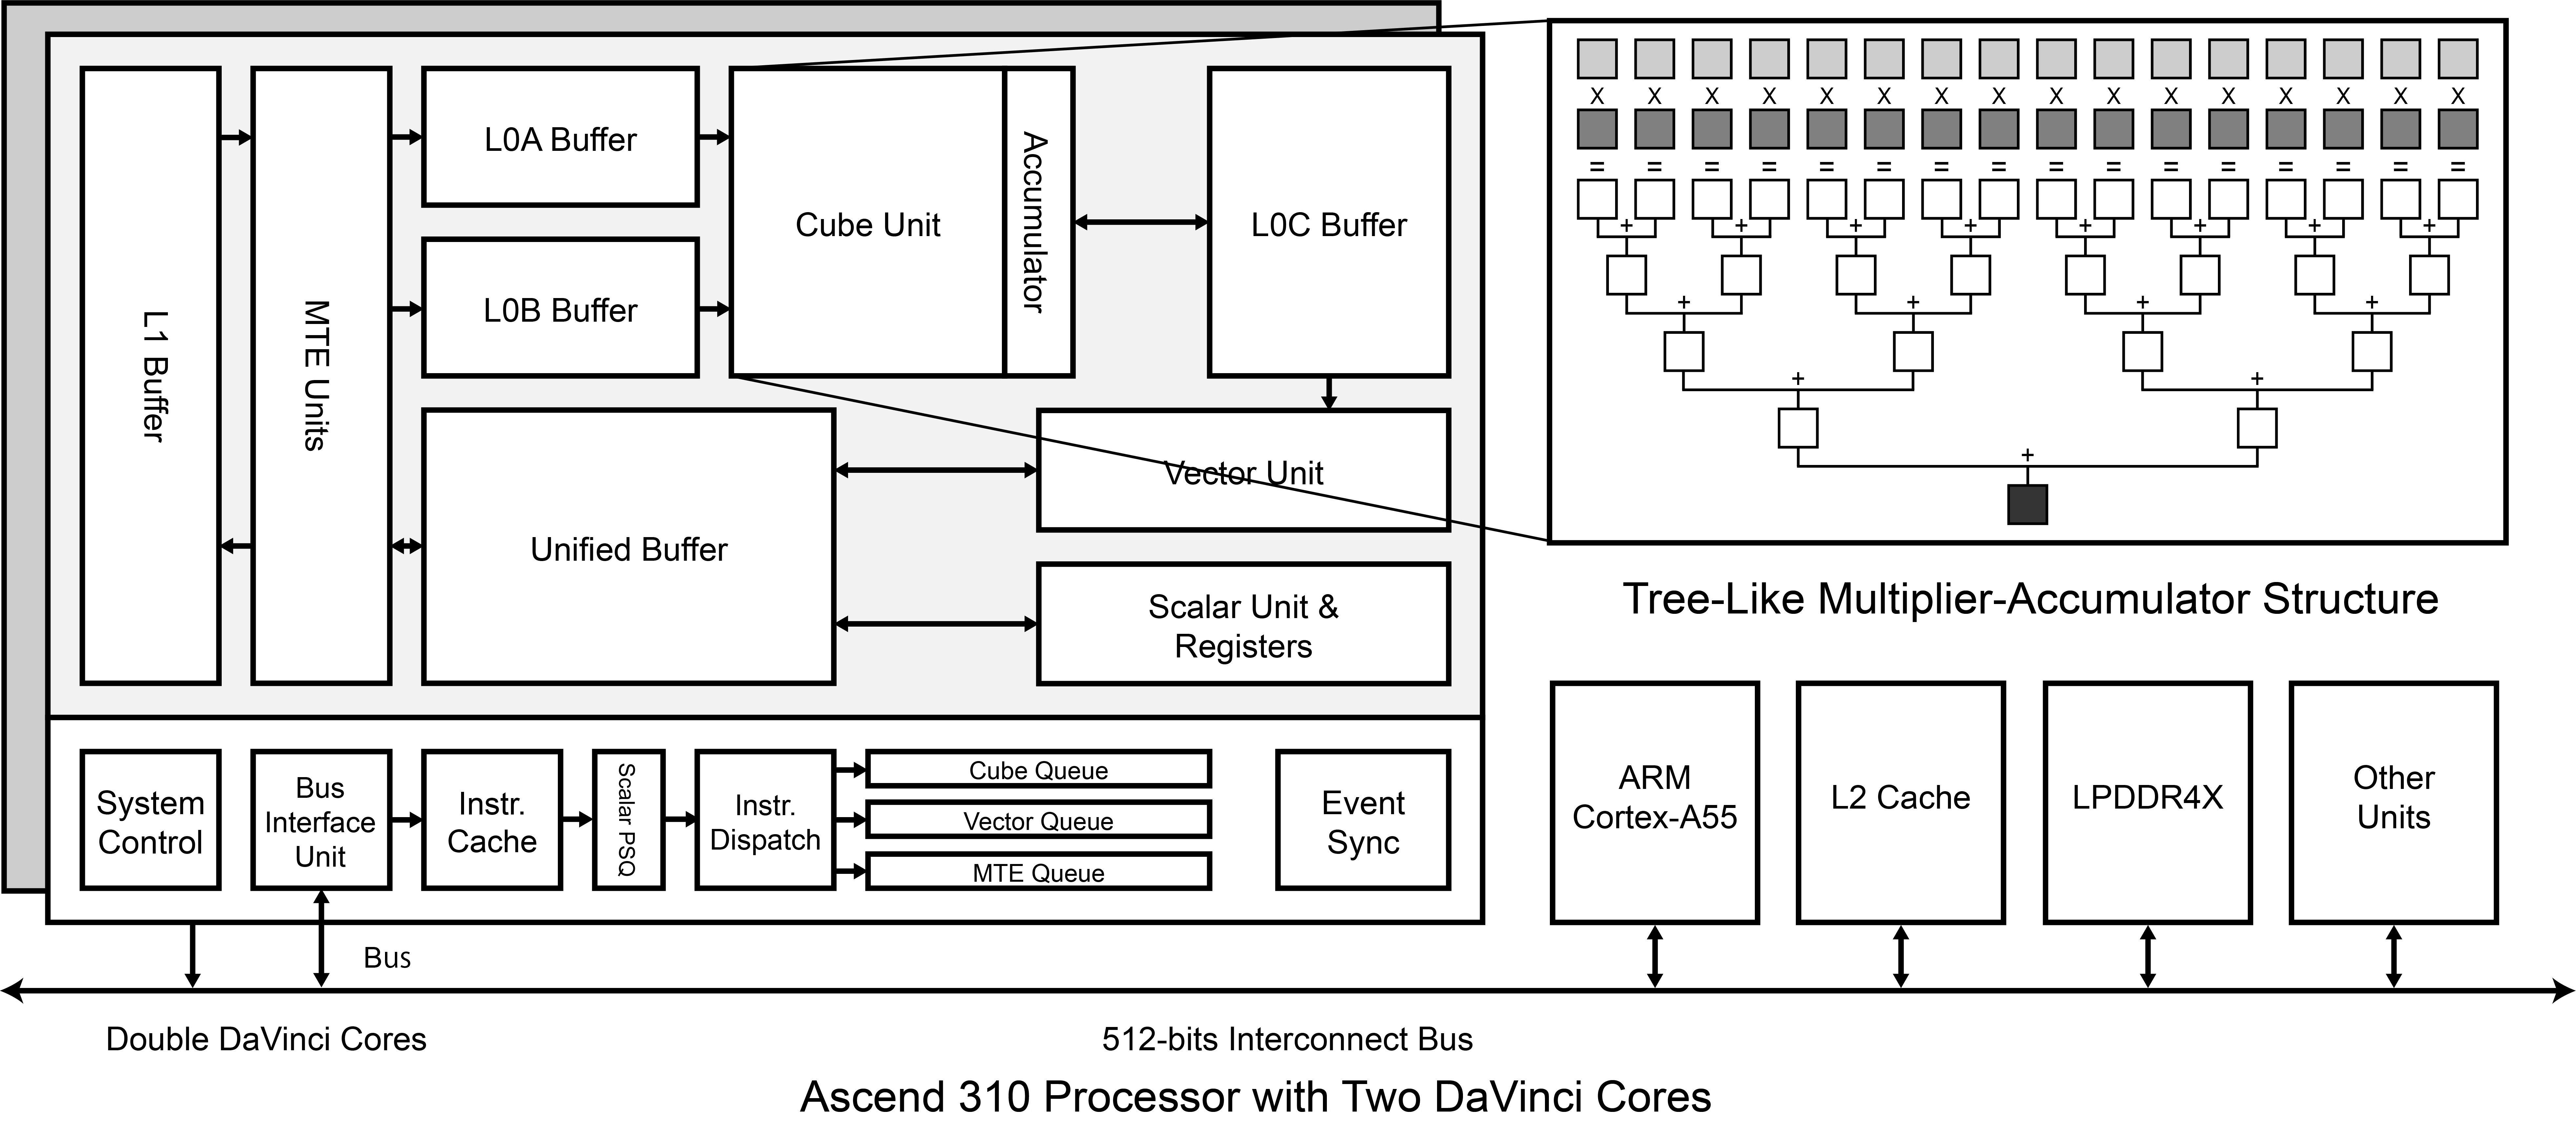
\includegraphics[scale=0.20]{figures/davinci_sub.png}}
    \caption{The hardware structure of an Ascend 310 processor}
    \label{fig:a310}
    \end{figure}

The compute units within the DaVinci Core include the Scalar Unit, Vector Unit, and Cube Unit. The Scalar Unit mainly handles address calculations and conditional branching, while the Vector Unit performs vectorized arithmetic or logical operations, such as data preprocessing and activation functions. At the heart of the DaVinci Core is the Cube Unit, which enhances the efficiency of matrix multiplications. Each Cube Unit consists of 4096 FP16 MACs and 8192 INT8 MACs, organized as a $(16 \times 16)$ tree-like structure of multiplier-accumulators, as shown in Figure \ref{fig:a310}. Matrix multiplications are divided into multiple smaller units of $(16 \times 16 \times 16)$ for processing, with intermediate results accumulated in the L0C Buffer.

The storage units encompass external and internal storage, as well as Memory Transfer Engines (MTEs) that manage data paths. External storage includes L2 Buffer, DDR, and other storage accessed via the bus, while internal storage comprises five primary buffers (L1, L0A, L0B, L0C, and the Unified Buffer) and various registers. The MTEs (MTE1, MTE2, MTE3, and PIPE\_FIX for Ascend 910B only) control data transfer between these internal storage buffers. These five buffers and MTEs work together to bridge the gap between lower memory bandwidth and high compute speed.
        
The control units manage the coordination between compute and storage units and consist of System Control, the Scalar Program Scheduling Queue (PSQ), Instruction Dispatch, instruction queues (for Cube, Vector, and MTE operations), and Event Synchronization. The Scalar PSQ receives and decodes instructions from the Instruction Cache, and Instruction Dispatch then routes these instructions to the appropriate queues. Event Synchronization handles data dependencies, ensuring correct execution order using a binary semaphore mechanism with eight registers. For Ascend 910B, an additional inter-core synchronization mechanism, based on a slower global memory-supported semaphore, is used to manage coordination across multiple cores.

\begin{figure}[tb]
    \centering{\includegraphics[scale=0.26]{figures/ascend.png}}
    \caption{The logic diagrams of Huawei Ascend 310 and 910B hardware structure}
    \label{fig:dav}
    \end{figure}

One major difference in hardware structure between Ascend 310 and Ascend 910B lies in how Cube Units connect with Vector Units. Figure \ref{fig:dav}(a) shows that Ascend 310 features a direct data path between the L0C Buffer and the Unified Buffer, facilitating efficient data transfer from Cube Units to Vector Units. In contrast, Ascend 910B lacks this direct path; instead, Cube and Vector Units must interact through global memory, which decouples these computation units. Consequently, Ascend 910B has a single Cube Core supporting multiple Vector Cores, as illustrated in Figure \ref{fig:dav}(b). This configuration changes the one-to-one mapping of Cube and Vector Units in Ascend 310 to a one-to-many mapping in Ascend 910B.

Although Ascend 910B's design allows greater flexibility by supporting multiple Vector Cores per Cube Unit, the reliance on global memory for data exchange introduces additional latency, potentially offsetting the benefits of increased parallelism. The design differences mean that Ascend 310's configuration may offer more efficient synchronization and data flow within a single core, while Ascend 910B's structure provides scalability but incurs higher data communication costs.

\subsection{Exploration and Optimization on AI processors}
\label{Sec:1_1_3}

With the rapid development of AI processors, researchers have shown growing interest in understanding and optimizing this novel hardware across various domains. Similar to previous efforts focused on traditional GPUs \cite{DBLP:conf/ppopp/ZhangTXLZC17}, researchers have initiated detailed investigations into AI processor architectures, such as Tensor Cores \cite{DBLP:journals/corr/abs-1804-06826}. These investigations have facilitated performance modeling on AI processors, typically divided into two main approaches: white-box and black-box models. White-box models require in-depth knowledge of the hardware, offering high interpretability but limited generalizability across different architectures \cite{DBLP:conf/ispass/RaihanGA19}. Conversely, black-box models rely on historical performance data, requiring little to no hardware-specific information and allowing for broader application, albeit at the cost of reduced transparency \cite{DBLP:conf/nips/ChenZYJMCGK18, DBLP:journals/corr/abs-2008-01040}.

Optimization research on AI processors generally follows two main directions. The first focuses on improving the efficiency of core AI operations, particularly matrix multiplications, which are central to most AI workloads \cite{gccblas, oneapi, 9820727, 9139835}. This research aims to fully leverage the native strengths of AI processors by refining computational techniques, optimizing memory access patterns, and improving data management to reduce latency and maximize throughput.

The second research direction explores ways to expand the application scope of AI processors, adapting them for general-purpose computations beyond AI-specific tasks. For example, some studies have adapted reduction and scan operations to Matrix MACs on Nvidia GPUs by segmenting data and processing it across warps and blocks within the CUDA compute hierarchy \cite{DBLP:conf/sccc/CarrascoVN18, DBLP:conf/ics/DakkakLXGH19}. Other work has focused on designing dense matrix multiplication techniques tailored to narrow matrix operations, which significantly enhances Matrix MAC utilization \cite{DBLP:conf/ic-nc/TangK0K20}, or applied matrix multiplications for polynomial convolutions in lattice-based cryptography \cite{DBLP:journals/access/LeeSZH22}. Additionally, research by Hu \textit{et al.} \cite{10.1145/3514221.3517869} investigated using Matrix MACs to accelerate join operations in database processing. These efforts typically involve restructuring data layouts and computation hierarchies to align with the architectural strengths of Matrix MACs, thereby increasing utilization and demonstrating the versatility of AI processors for non-AI applications.

Overall, these studies underscore the potential for AI processors to play a broader role in high-performance computing. By extending their application range through innovative adaptation techniques, researchers continue to explore the boundaries of what AI processors can achieve beyond their primary design.

\section{Motivations}
\label{sec_1_2_motivations}

\subsection{Hidden Hardware Details of AI Processors}

Although hardware manufacturers have published various architectures for AI processors, the public and research community remain largely unfamiliar with these hardware specifics beyond a few general parameters, such as FLOPS. These high-level specifications offer only a broad overview of hardware performance, lacking the detailed information needed for effective algorithm migration and optimization. One reason for this knowledge gap is that most AI processors are not available as consumer-grade physical products but are primarily accessible through cloud platforms. Consequently, performance evaluations conducted in virtualized cloud environments are often influenced by resource-sharing policies, potentially leading to inaccurate assessments that obscure architectural details.

Another factor contributing to this unfamiliarity is the limited functionality of toolchains provided for most AI processors. Many toolchains restrict access to high-level APIs, typically integrated within deep learning frameworks, which prevent developers from performing instruction-level benchmarks to analyze essential hardware characteristics such as bandwidth and throughput. Table \ref{tab:sec_1_2_table_1} outlines the availability and API level provided by various popular AI processor manufacturers.

\begin{table}[tbp]
    \caption{Availability and API level of AI processor manufacturers}
    \label{tab:sec_1_2_table_1}
    \begin{center}
    
    \scalebox{0.85}{
        \begin{tabular}{c|c|c}
        \toprule[1pt]
            \textbf{Manufacturer} &
            \textbf{\makecell[c]{Public Availability}} &
            \textbf{API Level} \\
        \midrule[0.5pt]
    
        \makecell[c]{Qualcomm} &
        \makecell[c]{Mobile SOC \cite{HDSP}} &
        \makecell[c]{Operations in QNN \cite{QNN}}
        \\
        \midrule[0.5pt]
    
        \makecell[c]{Google} &
        \makecell[c]{Cloud platforms \cite{DBLP:conf/isca/JouppiYPPABBBBB17}} & 
        \makecell[c]{Operations in TensorFlow or \\ PyTorch XLA \cite{XLA}}
        \\
        \midrule[0.5pt]
    
        \makecell[c]{Cambricon} &
        \makecell[c]{Cloud platforms \cite{DevP}} &
        \makecell[c]{Low-level C \& assembly \cite{BANG}}
        \\
        \midrule[0.5pt]
    
        \makecell[c]{Nvidia} &
        \makecell[c]{Physical cards \cite{ADA}} &
        \makecell[c]{Low-level CUDA \& PTX \cite{PTX}}
        \\
        \midrule[0.5pt]
    
        \makecell[c]{Baidu} &
        \makecell[c]{Internal usage} &
        \makecell[c]{Applications in Baidu AI Cloud \cite{Pad}}
        \\
        \midrule[0.5pt]
    
        \makecell[c]{Huawei} &
        \makecell[c]{Physical cards \cite{DBLP:conf/hotchips/LiaoTXZ19}} &
        \makecell[c]{Low-level C \& assembly \cite{CANN}}
        \\
    
        \bottomrule[1pt]
        \end{tabular}
    }
    
    \end{center}
    \end{table}

In contrast to Nvidia GPUs, which have been extensively studied \cite{DBLP:journals/corr/abs-1804-06826, DBLP:conf/ppopp/ZhangTXLZC17, DBLP:conf/ics/ZhouTZWS17, DBLP:conf/ispass/RaihanGA19, DBLP:conf/pldi/HongSKRKPRS18, DBLP:conf/cgo/ZhouMSM21}, the limited transparency in AI processor details poses significant challenges for algorithm migration and optimization. For example, when implementing a matrix multiplication of size $(256 \times 256 \times 256)$, Huawei Ascend processors require more loop iterations to execute the operation compared to Google TPUs, since the Ascend's Matrix MAC size $(16 \times 16)$ is considerably smaller than that of the TPU $(128 \times 128)$. This discrepancy necessitates different tiling parameters for optimal performance. Without access to such hardware details, programmers are unable to determine the most efficient tiling strategies, making algorithm optimization highly challenging.

To address this gap, this thesis begins with a comprehensive dissection of the Huawei Ascend AI processor, utilizing various benchmarks to uncover its specific hardware characteristics.

\subsection{Inefficient Hardware Units on AI Processors \label{sec_1_2_2}}

\begin{figure}[tbp]
    \centering{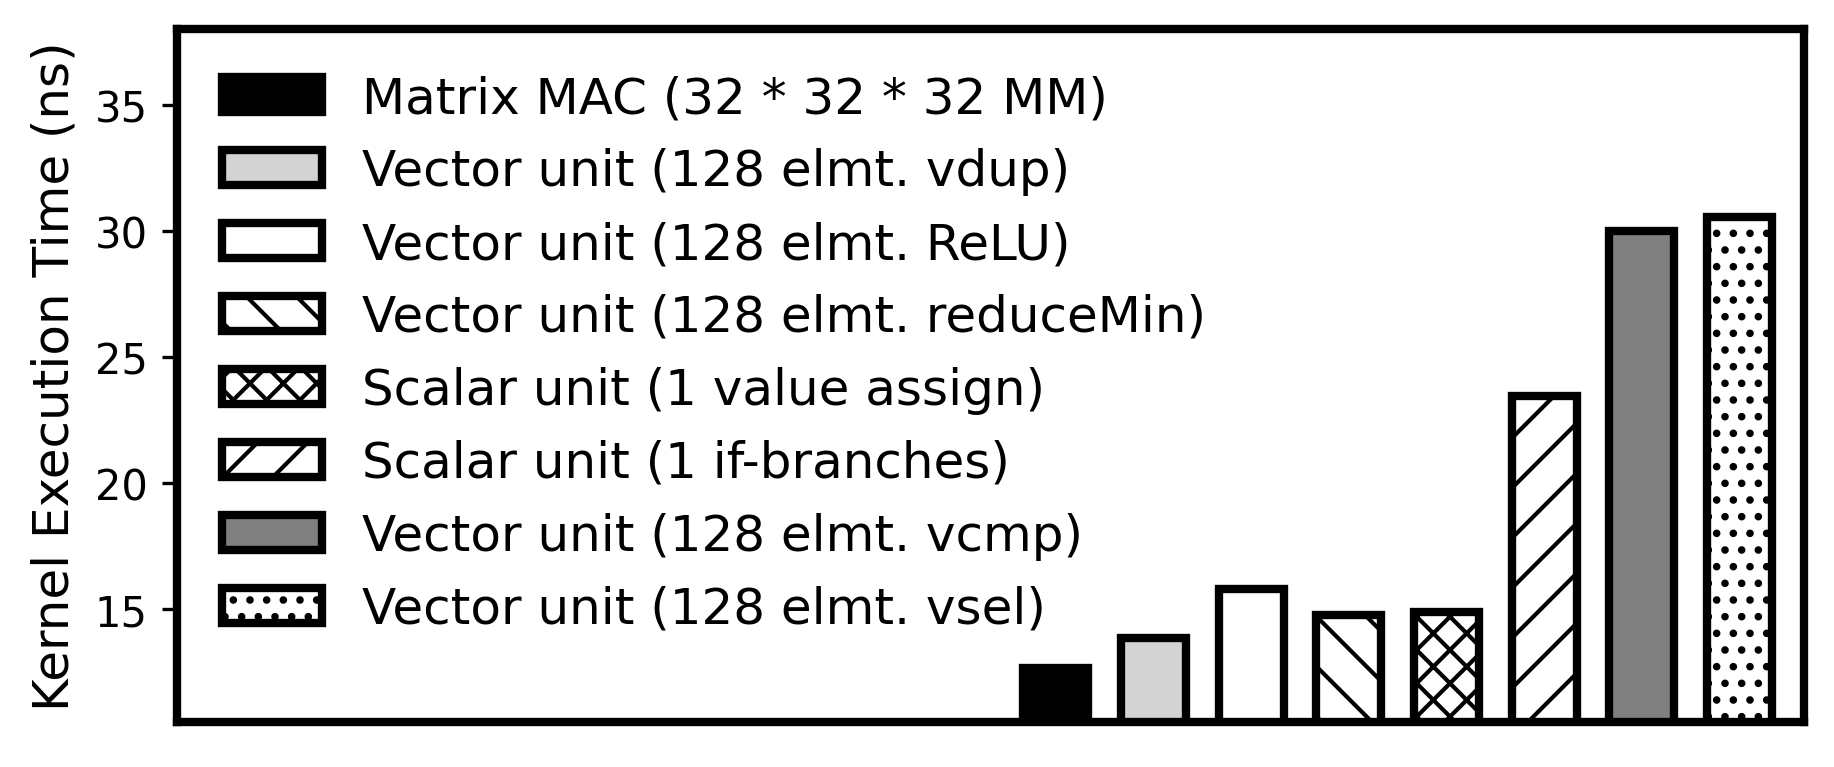
\includegraphics[scale=0.75]{figures/background_data.png}}
    \caption{The benchmark results on Huawei Ascend 310 AI processors}
    \label{fig:benchmark}
    \end{figure}

As standalone processors, AI processors are equipped with additional units beyond Matrix MACs to support necessary operations, such as instruction dispatch and vectorized computation. As discussed in Table \ref{tab:sec_1_1_table_1}, aside from GPUs, most AI processor designs prioritize hardware resources for enhancing matrix multiplication performance, often at the expense of other units.

To examine the efficiency of these additional units on the Huawei Ascend 310 AI processor, we conducted an instruction-level benchmark. Each test involves repeated executions of specific operations, such as a $(32 \times 32 \times 32)$ matrix multiplication for the Matrix MACs, 128-element ReLU operations for the vector units, and single-operand if-branch instructions for the scalar units. By increasing the number of operations in each test, we derived the execution time per individual instruction based on the measured increase in total execution time.

Figure \ref{fig:benchmark} shows the benchmark results. A scalar conditional branch (if-branch) operation exhibits significantly lower efficiency, taking on average 1.48 $\times$ longer than a vectorized \verb|ReLU| operation, 1.69 $\times$ longer than \verb|vecDup|, and 1.60 $\times$ longer than \verb|reduceMin| on 128 elements in parallel. An immediate assignment operation in scalar units takes approximately 0.94 $\times$ the execution time of \verb|ReLU|, despite \verb|ReLU| involving data read, compute, and write operations. Vectorized comparison and selection operations (\verb|vcmp| and \verb|vsel|) are particularly inefficient, taking 1.90 $\times$ and 1.93 $\times$ longer than \verb|ReLU|, respectively.

These findings highlight the limited efficiency of non-MAC units, particularly for scalar and certain vectorized operations. This hardware design constraint poses challenges for migrating traditional algorithms from other platforms to AI processors. Even with successful migration, implementations often suffer from significant performance degradation due to the limited efficiency of these auxiliary units.

\subsection{Low Usage Rate of Matrix MACs}

Since Matrix MACs in AI processors are designed exclusively for matrix multiplications, many algorithms and applications cannot fully leverage this high-performance hardware. Even for algorithms that inherently involve matrix multiplications, the actual usage rate of Matrix MACs is often lower than expected.

\begin{figure}[tbp]
    \centering{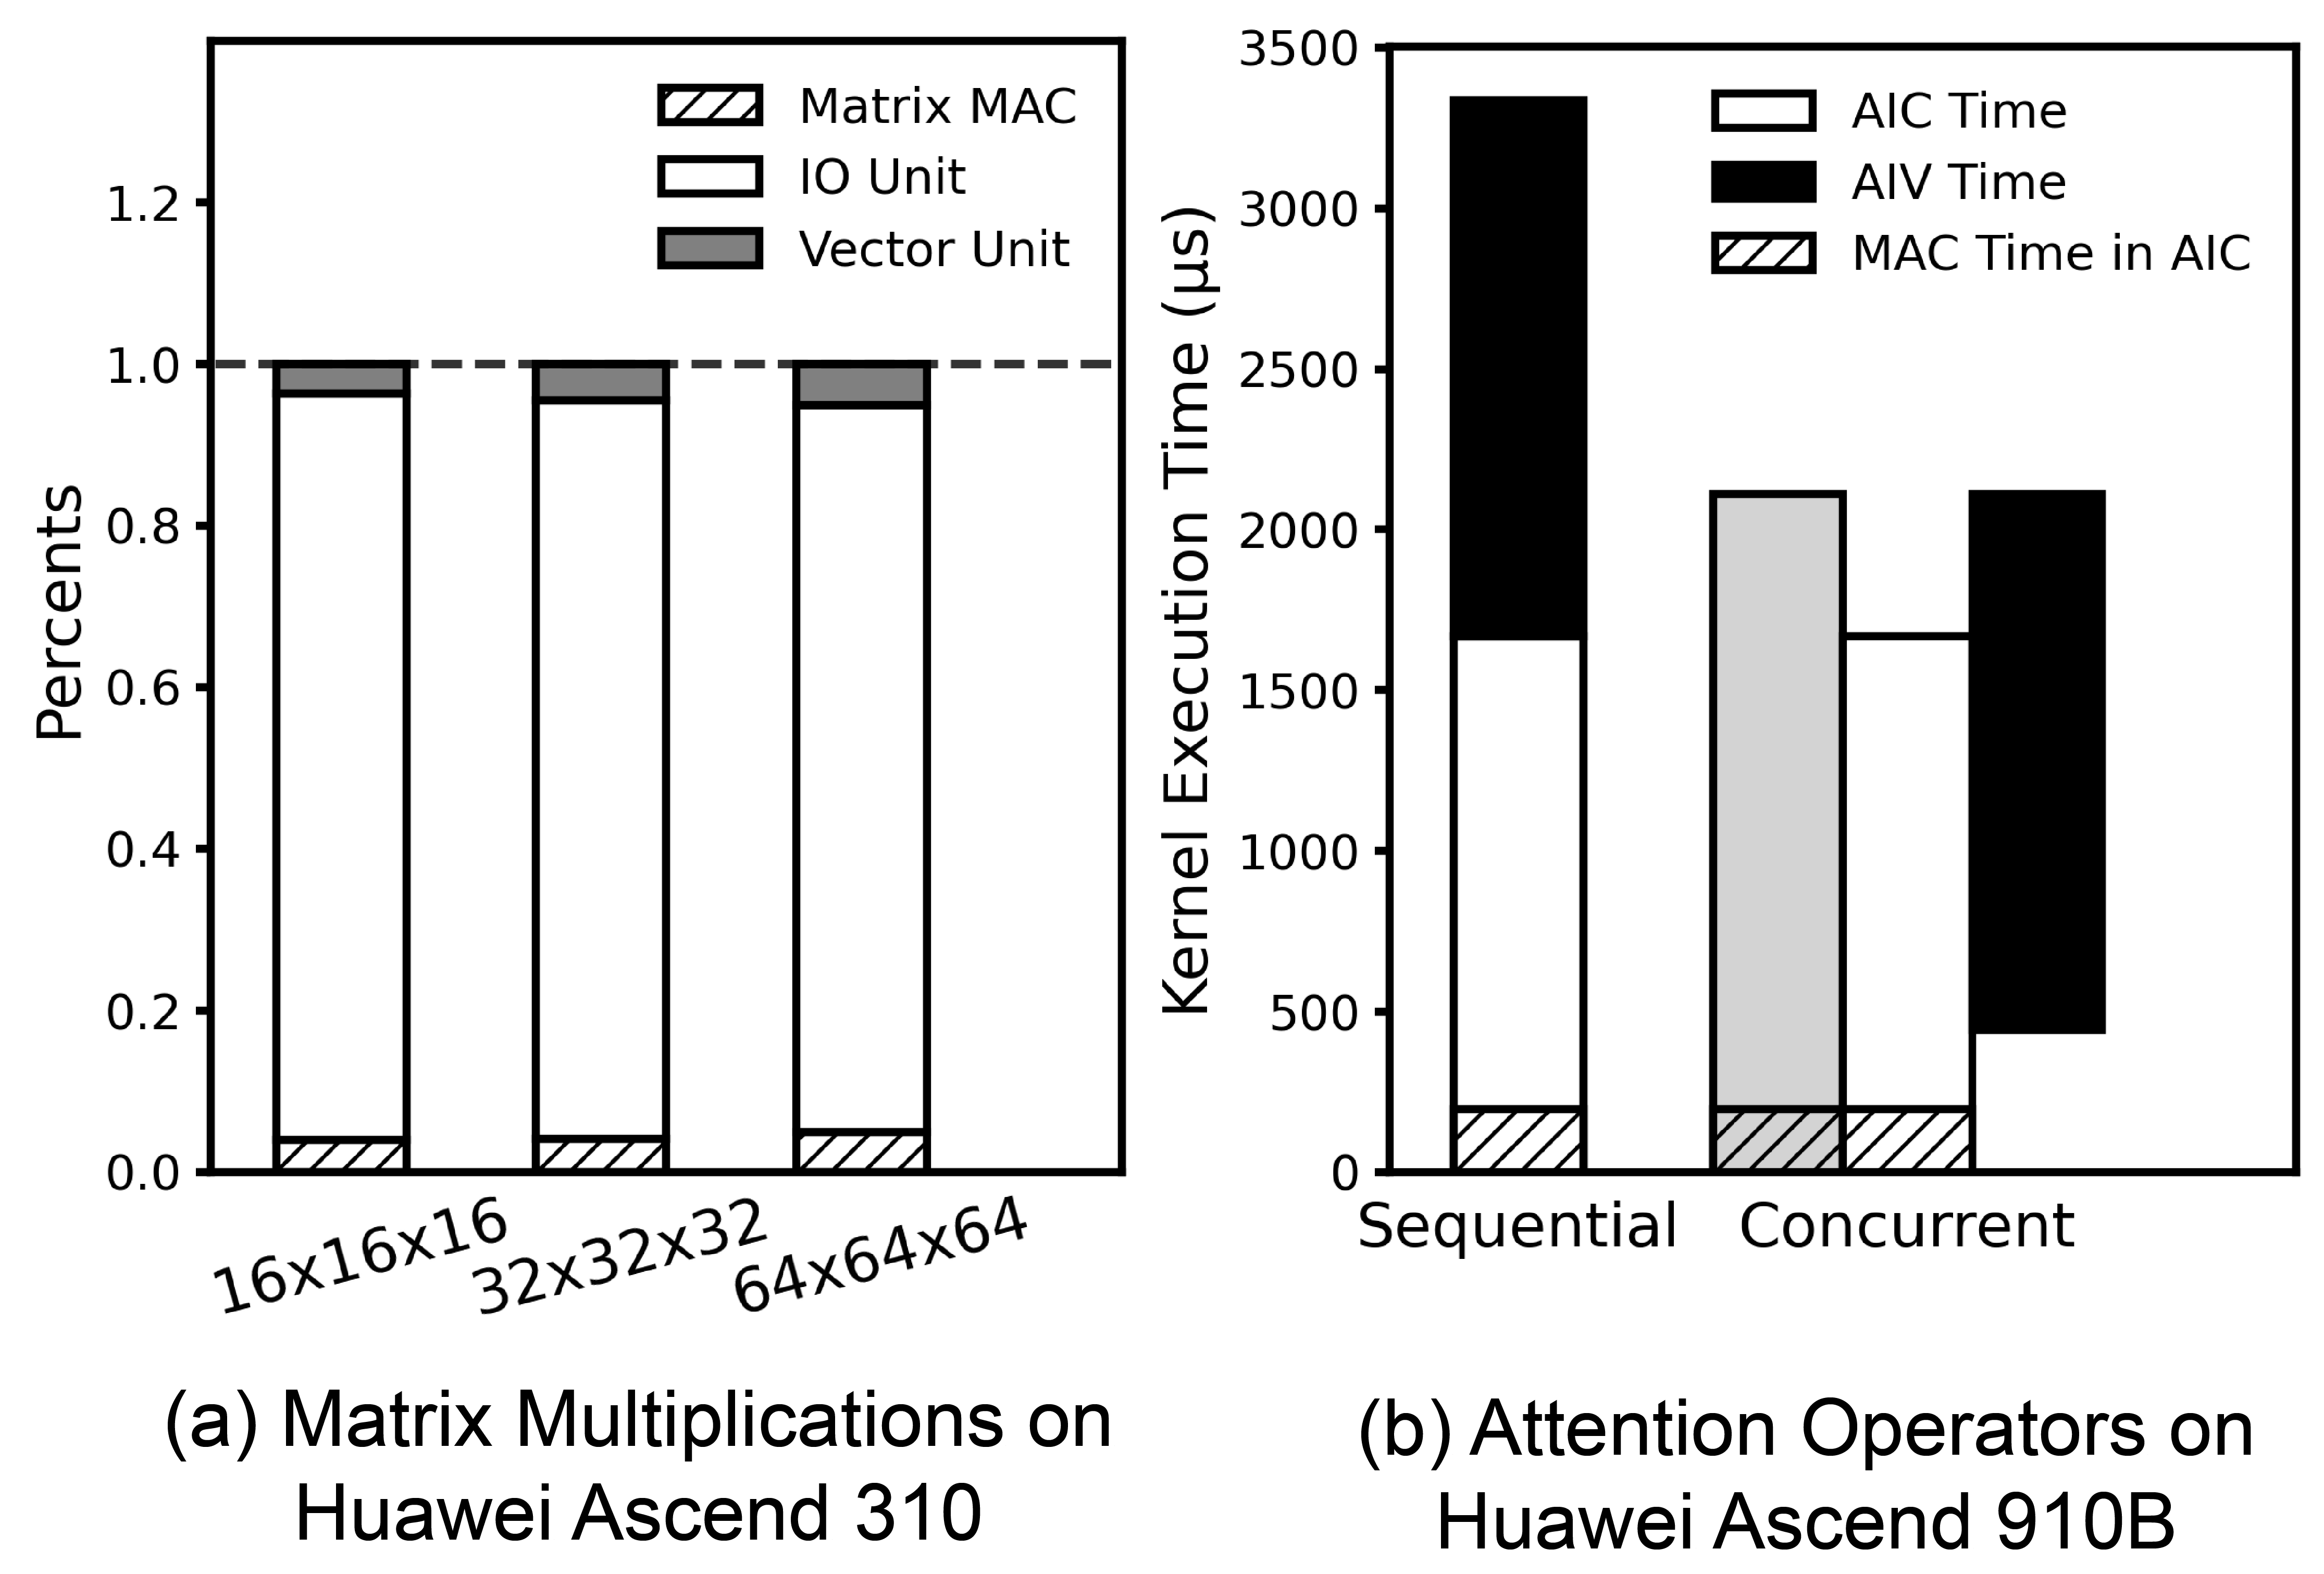
\includegraphics[scale=0.25]{figures/background_flash.png}}
    \caption{The percents of matrix multiplication rates on Ascend 310 and 910B processors}
    \label{fig:back_flash}
    \end{figure}

Previous studies and official documentation \cite{moustafaaccelerating, cann_sugg} have highlighted the underutilization of Cube Units and the limited performance of Vector Units in Ascend 310. To further investigate this issue, we evaluated two representative applications on Ascend processors: matrix multiplications on Ascend 310 and attention operations on Ascend 910B \cite{DBLP:conf/nips/VaswaniSPUJGKP17}. These tests provided insight into the performance of Matrix MACs across different matrix dimensions.
    
Figure \ref{fig:back_flash}(a) presents the results for matrix multiplications of various sizes on Ascend 310, showing a consistently low utilization rate of Matrix MACs (below 5\%). For Ascend 910B, the evaluation includes a breakdown of execution times for Cube Units (denoted as AIC Time) and Vector Units (denoted as AIV Time). As shown in Figure \ref{fig:back_flash}(b), AIC Time represents the execution time dedicated to matrix multiplications, which is comparable to the results observed on Ascend 310. Even though the attention operation involves substantial matrix calculations, such as $(128 \times 128 \times 128)$ and $(256 \times 128 \times 256)$ multiplications, the Matrix MAC usage rate remains low in both naive sequential and optimized concurrent executions.

These results indicate that on both Ascend 310 and Ascend 910B processors, Matrix MACs are not fully utilized, even in applications that are heavily reliant on matrix multiplications. This underutilization suggests potential opportunities for developing more efficient algorithms that can better exploit the cooperative capabilities of multiple units.

\section{Main contributions}
\label{sec_1_3_contributions}

\subsection{Performance Modeling on Huawei Ascend}

We begin by demystifying the Huawei Ascend 310 processor through micro-benchmarks that reveal key characteristics of the DaVinci Core, which serves as the central AI processing unit in the Huawei Ascend architecture. Particular focus is placed on the IO units, as they play a critical role in influencing execution time. Our analysis examines how the Memory Transfer Engines (MTEs) manage and compete for data paths that connect the separate memory units. In addition to benchmarks evaluating bandwidth sharing and contention ratios, we designed specialized benchmarks to identify the sources of contention, primarily the Interconnect Bus, and to analyze its runtime behavior under contention.

Building on these insights, we developed a discrete-event-based performance model, \textbf{Verrocchio}. Verrocchio captures essential architectural features critical to DaVinci Core performance, including bandwidth contention and concurrent execution of hardware units with synchronization. Evaluation results demonstrate that Verrocchio achieves average error rates of 2.62\% and 2.30\% for single-core and dual-core executions of sample kernels, respectively. By leveraging Verrocchio, we optimized a matrix multiplication algorithm, enabling search space exploration in tiling size selection. This optimization achieved a speedup of 1.70$\times$ at the operator level and 1.53$\times$ at the application level compared with CANN's \cite{CANN} native operators, with prediction error rates of 5.06\% and 5.25\% for single-core and dual-core execution, respectively.

\subsection{(1) Replacing Inefficient Operations}

\textbf{SelB-\textit{k}-NN} (\textbf{Sel}ection-\textbf{B}itonic-\textbf{\textit{k}}-\textbf{NN}) is a mini-batch \textit{k}-nearest neighbors algorithm optimized for high-performance AI processors. For each mini-batch, SelB-\textit{k}-NN incorporates an efficient distance computation step alongside a specialized \textit{k}-selection method. Inspired by selection sort, SelB-\textit{k}-NN employs a bitonic 1-selection technique to maintain the min-\textit{k} result array, comparing minimized values of the computed distances with the initial element of this array \cite{DBLP:conf/sigmod/ShanbhagPM18}. Compared to previous approaches, SelB-\textit{k}-NN minimizes the reliance on hardware-inefficient scalar operations and vectorized comparisons \& selections.

To enhance portability across different AI processor architectures, we designed SelB-\textit{k}-NN with minimal hardware dependencies. Only basic operations like \verb|vecDup|, \verb|ReLU|, and \verb|reduceMin| (\verb|reduceMax|), without indexing, are required, ensuring compatibility with most AI processors. For all mini-batches, an early exit policy dynamically reduces \textit{k}-selection workloads, and our quantification shows that this workload reduction is inversely proportional to the data size. We formulated the tiling shape selection as an optimization problem, aiming to improve SelB-\textit{k}-NN's overall performance. Additionally, an offline pruning method was introduced during preprocessing to reduce the search space of the optimization problem.

\subsection{(2) Mapping Computations to Matrix Multiplications}

\textbf{Cube-}$\mathbf{fx}$ is a mapping technique that utilizes the computational power of Matrix MACs to parallelize Taylor expansion. Cube-fx is particularly effective when a dataset requires computation across multiple independent functions \cite{boyd2004convex, deller1993discrete, DBLP:conf/icpr/ManessiR18}. It formulates the construction and evaluation of Taylor polynomials as two consecutive matrix multiplications. While matrix multiplication for polynomial evaluation is straightforward, Cube-fx innovates in its approach to matrix generation. During this step, Cube-fx reads input data as contiguous memory segments from external memory, preparing it directly for computation based on Matrix MAC output.

Unlike previous optimization approaches for Matrix MACs, Cube-fx avoids extra matrix generation or data layout conversion, relying solely on a few small constant matrices. Based on precision requirements, Cube-fx adjusts the order of expansion to approximate the original functions effectively. For lower precision requirements, Cube-fx enhances data parallelism by combining inputs and coefficient matrices as direct sums, enabling multiple inputs to be computed within a single set of basic matrix multiplications. Cube-fx is adaptable across various AI processors and is particularly efficient on devices with high-speed communication between vector units and Matrix MACs.

\section{Thesis Organization}
\label{sec_1_4_organization}

The remainder of this thesis is organized as follows. Chapter 2 begins by presenting a detailed analysis and benchmarking of Huawei Ascend AI processors. It then introduces the performance model Verrocchio and provides a comprehensive evaluation of its accuracy. Chapter 3 explores the first optimization approach, which focuses on replacing inefficient scalar and vectorized operations with more suitable alternatives. Chapter 4 presents the second optimization approach, which involves mapping certain scalar and vectorized operations into matrix multiplications for enhanced performance. Finally, Chapter 5 concludes the thesis and outlines directions for future research.